\chapter{Background}\label{sec:background}

\section{Overview}
\paragraph{}
The ROME interface is built on the Perl Catalyst MVC framework using a Template::Toolkit view and a MySQL Model. The analysis is performed in R using many of the tools available from the Bioconductor project.

\section{Design Decisions}

\subsection*{Web-Application}
\paragraph{}
A web-based client-server design was chosen over a standalone piece of software for two main reasons:

\paragraph{}
Firstly, running the software on a server means that the end users do not have to be concerned with keeping their software up to date. This is particularly important because both R and Bioconductor are under constant development and so must be updated frequently. As R and Bioconductor are modular it is also simpler to ensure dependencies are met on a central server than it is on a number of standalone installations. The alternative would be to take a snapshot of R and Bioconductor and distribute that as part of a monolithic application. Unfortunately, as many of the newer modules, to which the users require an interface, are dependent on the most recent stable versions of R and Bioconductor, a snapshot would rather defeat the point. 

\paragraph{}
Secondly, many of the analyses are computationally intensive. A standalone application would have to be run on a machine capable of processing, for example, large microarray experiments. This is not the type of processing power that biologists typically have to hand on their own desktop. Given this fact, most labs would presumably have to buy a dedicated box on which to run the analysis, in which case it makes more sense to have users connecting to this server as clients and running their analysis than physically sitting in front of the machine. 

\paragraph{}
A client-server model will also make it easier to extend the capacity of the analysis software by having the server delegate the processing to a computer farm. 

\subsection*{Perl}

\paragraph{}
Perl was initially selected for compatability with the European Bioinformatics Institute(EBI)'s Expression Profiler (EP) tool. After a few months of development it became clear that the low-level analyses we were interested in simply didn't fit well into the EP data model (which focuses more on clustering and dimension-reduction algorithms for multivariate analysis), so it made more sense to develop ROME seperately. That said, much of the code developed for EP was still of use, so it made sense to continue with Perl. Perl is a popular choice in bioinformatics applications due to its suitability as a glue language, its strong support for text parsing and the number of useful modules on CPAN (Comprehensive Perl Archive Network). This will make maintenance of ROME easier in the long term. 

\subsection*{Catalyst}

\paragraph{}
To begin with, ROME was developed from scratch, doing all its own session management, user management, access privileges and other basic framework functions. This was time-consuming to develop and debug. It was also my first development project and as such a steep learning curve. Much of the code written at the start of the project was less than ideally modular and easy to maintain. Eventually the decision was made to migrate to the new Catalyst Model-View-Controller (MVC) web-development framework \citep{web:catalyst}. Although this process took about a month, subsequent development was much faster as it left only the ROME-specific problems - managing and describing experiments, generating R scripts and so on. Catalyst provides the user and session management, and automates much of the basic CGI processing (extracting form values, URL mapping etc). Catalyst is also rapidly increasing in popularity and has many similarities to the already widely used Ruby-on-Rails framework, so finding people able to maintain ROME in the future will be much easier than if the entire application was custom built.

\subsection*{Open Source}

\paragraph{}
There are already a number of commercial software packages available for microarray analysis, including Agilent's GeneSpring and Stratagene's ArrayAssist. Clearly there is little point in developing a package in direct competition with these already successful tools. The aim of ROME is to provide an open-source solution. There have been many long debates on the relative merits of the open and closed source development models \citep{web:catb, web:eufloss}. There are obvious financial benefits to using free software, but this is not a primary concern as the sums of money involved in software acquisition are generally dwarfed by the costs of the necessary lab equipment for transcriptomics studies. Of greater potential benefit is the speed at which new algorithms could be made available to users with an open source development model. There has been a significant lag between the adoption of a method as \emph{de facto} standard in Bioconductor and the integration of that method into commercial software. The Bioconductor community has already demonstrated that it is capable of rapid production of useful and successful analysis algorithms using an open source model as seen in the previous chapter. It is hoped that they will be as proactive in developing interfaces to these tools once supplied with a framework to do so. 



\section{Catalyst}\label{sec:catalyst}

\paragraph{}
ROME was built with Catalyst (see section \ref{sec:catalyst}), a perl web developement framework. Data is stored in a MySQL database and statistical analysis is performed in R using the Bioconductor tools and some custom code. It has been designed such that adding new R scripts is a relatively simple process, allowing biologists to have rapid access to new bioconductor developments.

\paragraph*{}
A basic understanding of the framework on which ROME is based is required to understand the system. Catalyst (http://catalyst.perl.org) is a Model-View-Controller (MVC) web-framework written in Perl. MVC is a widely used standard pattern for designing web-applications. 

\begin{figure}[h]
\centering
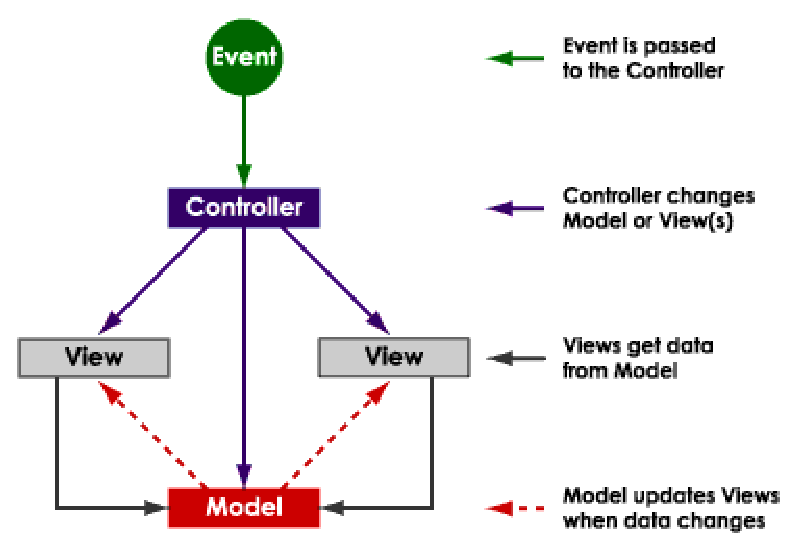
\includegraphics[scale=0.6]{images/mvc}
\caption{Model-View-Controller Pattern}\label{fig:mvc}
\end{figure}

\paragraph{}
The model,view and controller tiers can be considered as a variation on the more traditional input-processing-output paragdigm. The model is the processing layer, in the sense that it encapsulates the available data and the processes one can perform upon that data. The controller layer is analogous to the input as it deals with user requests, decides where to send them and asks the model to make appropriate changes or return appropriate information. The view deals with presentation of results to the user.


\subsection*{M}
\paragraph{}
The model tier deals with information processing, retrieving and altering information stored on the system. Typically, this will involve interacting with a database. There are a number of well-established Perl modules that provide a mapping between relational databases and perl objects, based on the standard DBI Database Interface module. These include Class::DBI and its extension Class::DBI::Sweet and the newer DBIx::Class. Catalyst has Model modules which are effectively just wrappers around these database mapping modules that plug them into the catalyst framework


\subsection*{V}
\paragraph{}
The view tier deals with presenting results to the user. For web development, this generally involves a templating system of some sort to insert the dynamic content into the static HTML outline of each page. Again, there are many modules on CPAN which provide templating functionality, including Mason, HTML::Template and the Template Toolkit. There are Catalyst wrappers to allow you to use all of these and more within the Catalyst framework.

\subsection*{C}
\paragraph{}
The controller deals with handling the application flow. In other words, it takes requests from the user (from the view), determines what to do with them, tells the model to make the appropriate alterations to the data, and passes on any results back to the user. The Controller layer is the heart of Catalyst and where it does most of the work. Model and View functions are mostly supplied by plugin modules, but in the Controller layer Catalyst does all the heavy lifting. 

\subsection*{}
\paragraph{}
The aim of the MVC pattern is seperation of concerns such that it is possible to change one layer of the application without affecting the others, for example changing the way in which the data is presented to the user via the view, or reusing the model in different applications. Generally an event causes a controller to change the model, the view or both. Changes to the model are automatically reflected in any dependent views. A more in depth discussion of the MVC pattern can be found in \citet{GOF}.

\subsection*{Catalyst processing} \label{sec:caturlmap}

\paragraph{}
Catalyst accepts http requests and forwards them on to one of the controllers as determined by the URL. The controller method will then take the request, retrieve or modify data in the model as requested and then return some result to be passed back to the user. Finally the controller will forward the result to the view. Catalyst determines which Controller is responsible for processing the request by URL mapping. For example the URL: \begin{verbatim}MyApp/Test/do_something/93\end{verbatim} 
might call the \verb|do_something| method of the Test controller with the argument 93. See section \ref{sec:caturlmap} for more details of URL mapping.

\paragraph*{}
Catalyst automatically creates a context object which is available everywhere in the application. This context object contains Catalyst::Request, Catalyst::Response, Catalyst::Config and Catalyst::Log objects (details of which can be found in their perldoc on http://search.cpan.org). This provides the controller with access to information about and content from the http request, details of the application configuration and a log for messages. Generally the response is handled by the view, but the controller may need access for setting cookies, redirects and so forth. The context object also contains a hash known as the stash, which provides place to store data to be shared between application components, primarily between the controller and the view.                                                                  


\subsection{Catalyst Controller Actions}

\paragraph{}
A Catalyst controller Perl module has \emph{actions} rather than \emph{methods}. An action is effectively just a method which has a rule defining the URLs to which it should be mapped. Catalyst has various types of actions, which differ in their URL matching rules:

\subparagraph*{Literal} \verb|sub foo : Path('/bar')| which match relative to their current namespace
\subparagraph*{Regex} \verb|sub foo : Regex(^item(\d+)/order(\d+)$)| which match any URL that matches the pattern. The match is not relative to the current namespace. 
\subparagraph*{RegexLocal} \verb|sub foo : RegexLocal(^widget(\d+)$)| which match any URL that matches the pattern. The match is relative to the current namespace.
\subparagraph*{Global} \verb|sub foo : Global{}| in which case the function name is mapped directly to the application base, for example http://localhost/foo
\subparagraph*{Local} \verb|sub foo : Local{}| in which case the function name is mapped relative to the current namespace.

\paragraph*{}
Full details of Catalyst's URL dispatching rules can be found from the Catalyst::Manual perldoc \citep{web:cpan}. 

\paragraph*{}
It is also possible to define \verb|Private| methods which are not mapped to a URL and may only be called internally using the Catalyst context object's \verb|forward| or \verb|detach| methods. Catalyst has a number of pre-defined private actions, called in pre-defined circumstances, that can be used or overridden in controllers:

\paragraph*{default}: Is the method called when nothing else matches. Generally this would be used to set a 404 (page not found) error back to the client. It can be defined in the base application module and will apply to other controllers unless specifically overriden.
\paragraph*{index}: Is the method called when the URL matches the base controller namespace.
\paragraph*{begin}: Called at the beginning of a request before any matching actions
\paragraph*{end}: Called at the end of a request                                                     
\paragraph*{auto}: Called at the beginning of a request and must return true for processing to continue.                                                                                                                   
\paragraph*{}
A flowchart of the Catalyst request cycle are shown in figure \ref{fig:cat_flow}.      

\begin{figure}[h]
\centering
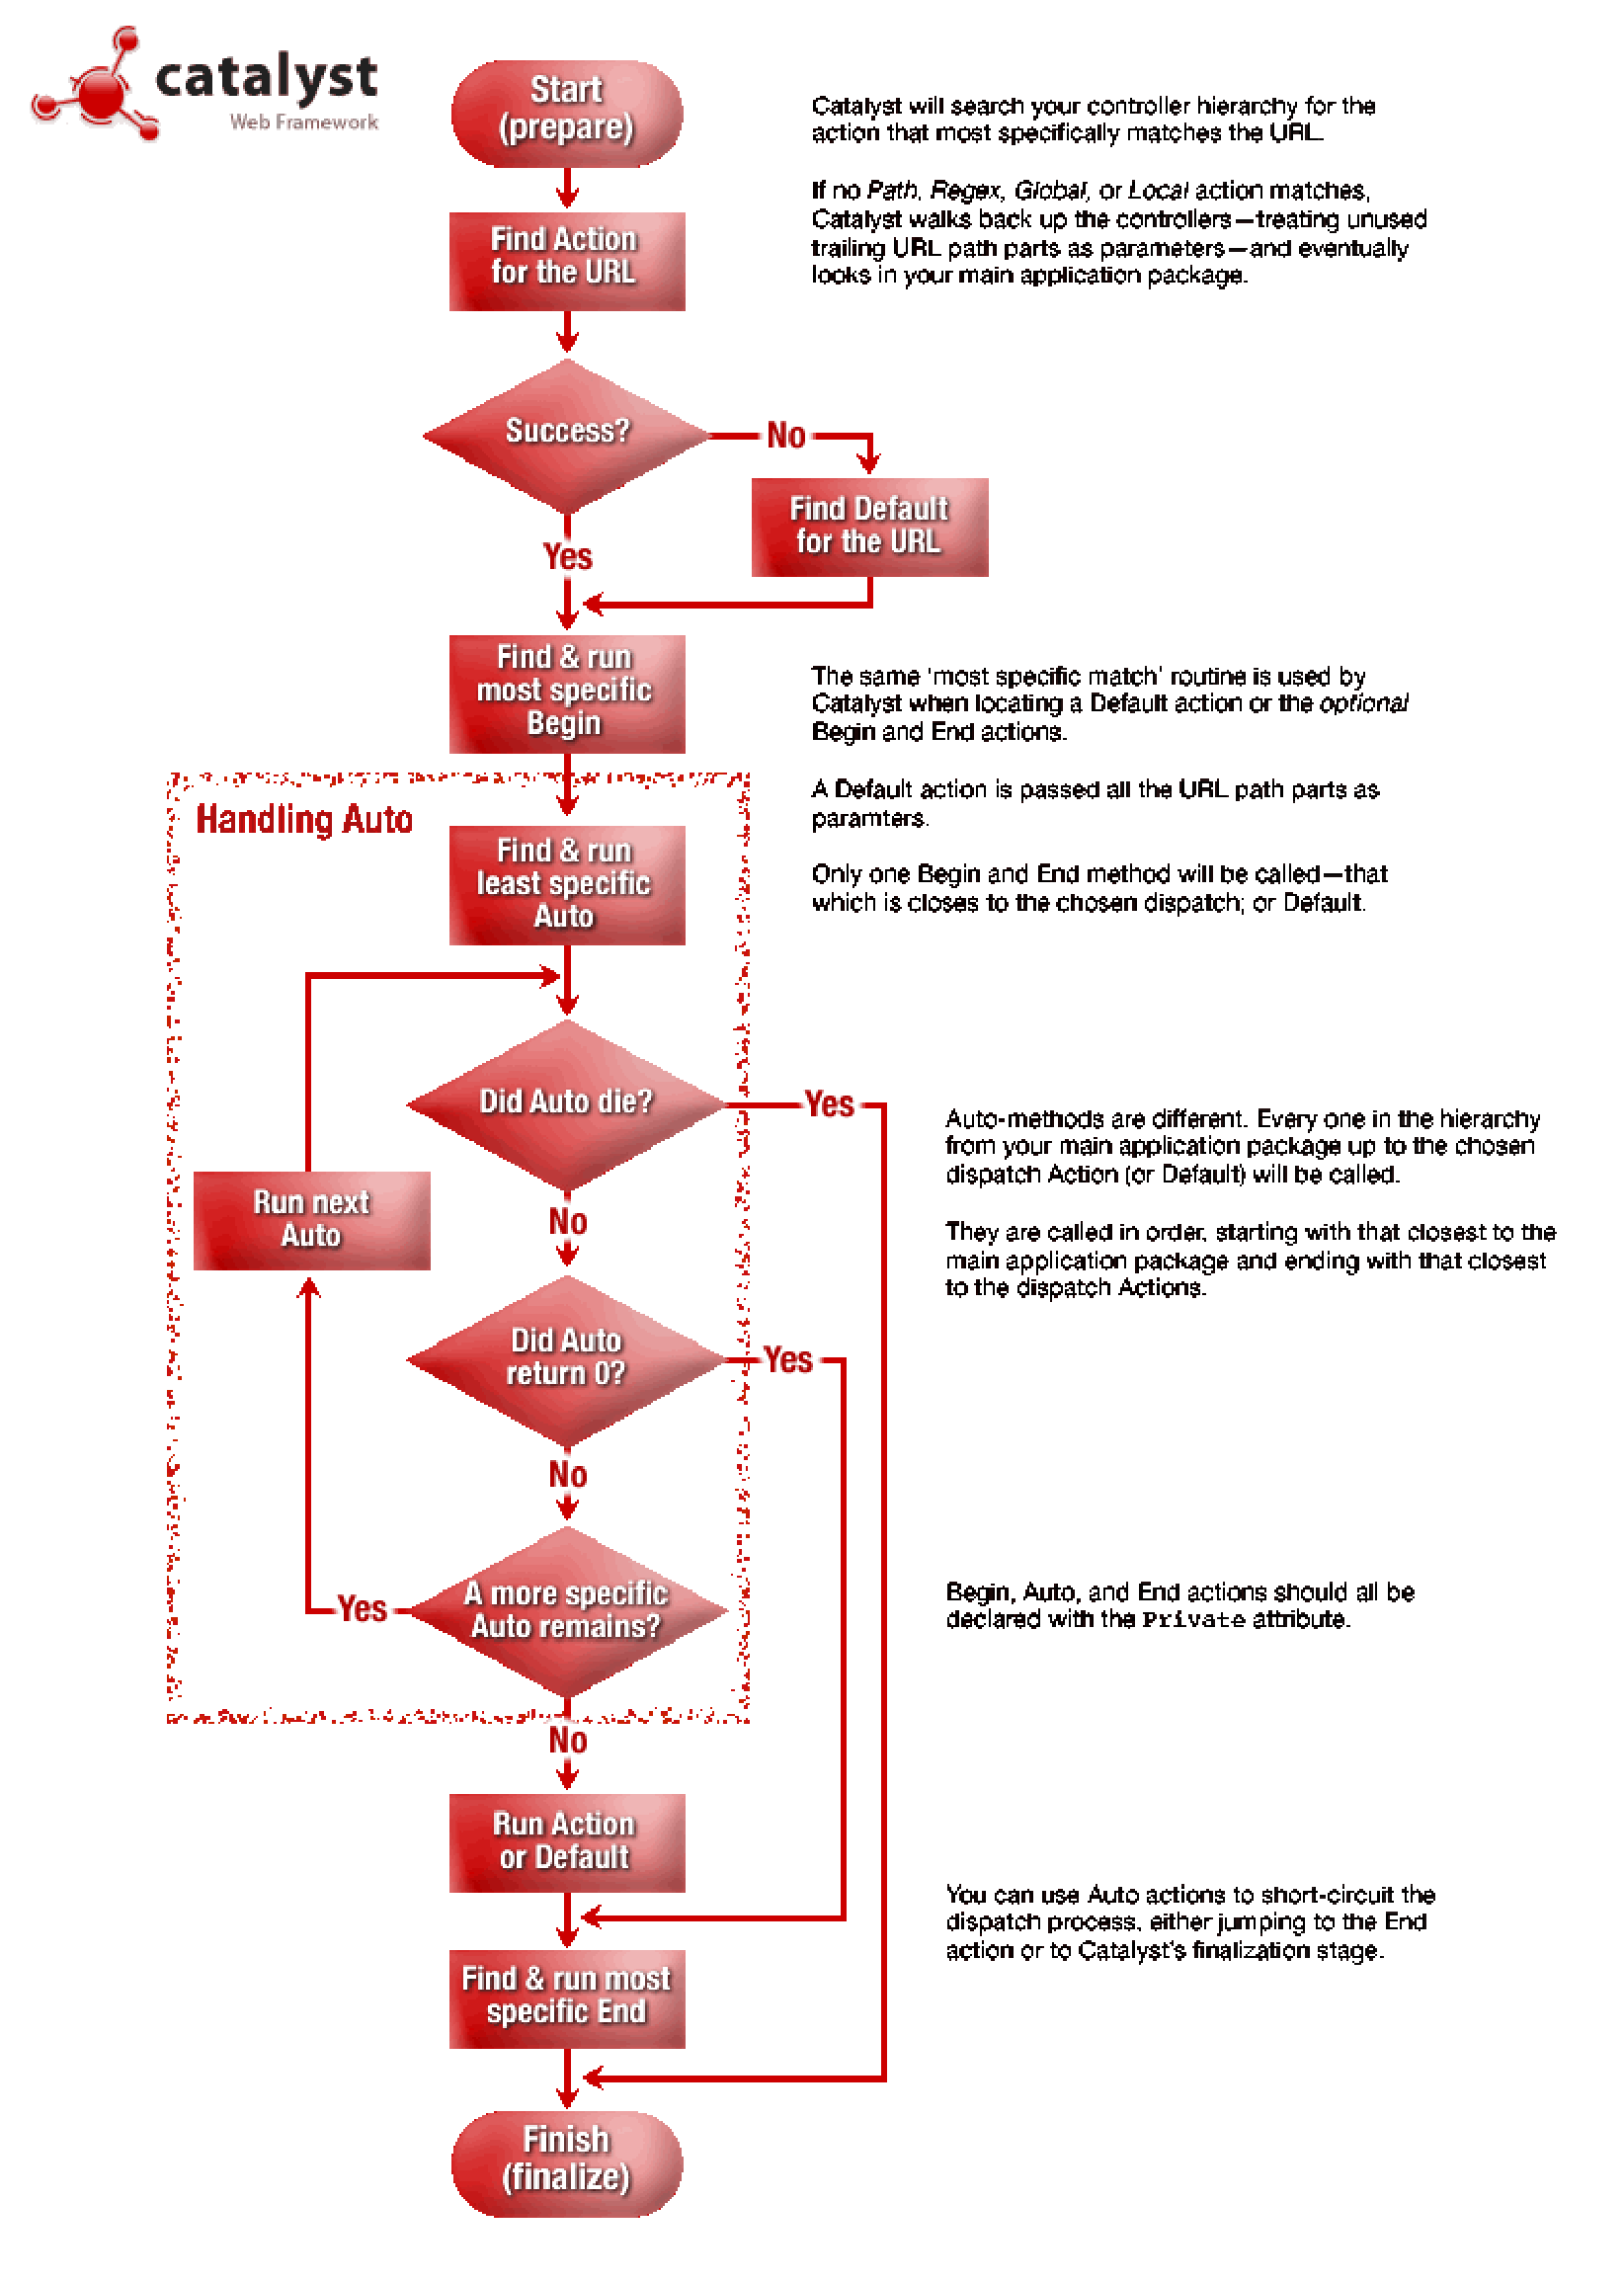
\includegraphics[scale=0.45]{images/catalyst-flow}
\caption{Catalyst Processing Flow}\label{fig:cat_flow}
\centerline{dev.catalyst.perl.org}
\end{figure}


\section{Sessions}
\paragraph{}
In order to store information between http requests, the Catalyst Session plugin is required. The session plugin adds a session to the the Catalyst context object. Data stored in the session hash is stored on the server and linked to a session key. The session key is also stored client-side, typically in a cookie. The client then sends the session key data along with each request and any data associated with that session key is restored to the session hash. The Session plugin requires two backend plugins to deal with the mechanics of storing data on the server and maintaining the session state on the client. There are a number of options in Catalyst, but ROME uses Session::State::Cookie and Session::Store::FastMmap. 

\section{Error Handling}

\subsection{Internal Server Errors}

\paragraph{}
In \verb|lib/ROME/Controller/Root.pm| 
If an exception occurs in a controller then the client either receives a suitably apologetic error page or, if the debug flag is on, a debug page with various bits of useful information. You can set an error message using \verb|$c->error($msg)| but this will only be displayed to the user if debug mode is on.

\paragraph*{}
You can use \verb|$c->log| to send information to the log if you wish. See the Catalyst::Log perldoc for details.

%% This should be in the catalyst core section.
% \subsection{User Errors}
% \paragraph{}
% Every template automatically gets an error\_msg field inserted before any other content (from \verb|root/src/site/layout|) into which you can put any messages you like by simply setting \verb|$c->stash->{error_msg}| in your action. If you only want to display the error and no other content, you can use the \verb|user_error.tt2| template, which is just an empty page with the title error.
% 
% \subsection{Form Validation Errors}
% Assuming you're using the Data::FormValidator plugin then you can include the dfv\_error.tt2 template prior to your form (see user/login.tt2 for an example). This template will format the error messages from the Data::FormValidator::Results object in \verb|$c->form| for you, so if your validation fails, you just return the form template and any errors will appear at the top (see the \verb|login| action in \verb|lib/ROME/Controller/User| for an example)





\section{Template::Toolkit}
\label{sec:tt}


